\documentclass{TIJMUjiaoanLL}
\pagestyle{empty}


\begin{document}


%课程名称
\kecheng{Linux系统概论}
%课程内容
\neirong{shell编程\ /\ 第13 \& 14章}
%教师姓名
\jiaoshi{伊现富}
%职称
\zhicheng{讲师}
%教学日期(格式:XXXX年XX月XX日XX时-XX时)
\riqi{2018年7月2\&9日10:00-12:00}
%授课对象(格式:XXX系XXXX年级XX班(硕/本/专科))
\duixiang{生物医学工程与技术学院2016级生信班(本)}
%听课人数
\renshu{28}
%授课方式
\fangshi{理论讲授}
%学时数
\xueshi{4}
%教材版本
\jiaocai{Unix入门经典,第1版}


%教案首页
\firstHeader
\maketitle
\thispagestyle{empty}

\mudi{
\begin{itemize}
  \item 掌握shell脚本的结构及其运行方法,shell脚本的注释、变量、特殊变量以及退出状态,shell脚本中流程控制的语法,shell脚本中函数的使用,常用的文件测试和比较运算符。
  \item 熟悉shell脚本从键盘读取输入的方法,输入输出重定向和命令替换的方法,脚本的调试。
  \item 了解shell函数的嵌套和递归、作用域。
  \item 自学shell脚本中数组的使用。
\end{itemize}
}

\fenpei{
\begin{itemize}
  \item (5')引言与导入:总结shell的职责,简单介绍shell脚本。
  \item (25')编程起步:讲解shell脚本的结构、运行方法、注释、变量使用、特殊变量和退出状态等基础知识。
  \item (20')流程控制:介绍流程控制的分类,讲解if-then、case等条件流程控制的逻辑流程和语法结构,讲解while、until、for等迭代流程控制的逻辑流程和语法结构,讲解常用的文件测试和比较运算符。
  \item (10')高级概念:总结输入输出重定向和命令替换的基本方法。
  \item (30')shell函数:讲解shell函数的声明与调用、返回值、嵌套和递归、作用域等相关知识,介绍数组的使用。
  \item (5')脚本调试:介绍对shell脚本进行调试的方法。
  \item (5')总结与答疑:总结授课内容中的知识点与技能,解答学生疑问。
\end{itemize}
}

\zhongdian{
\begin{itemize}
  \item 重点:shell脚本的结构、运行方法、变量等基础知识,shell脚本中的流程控制。
  \item 难点:shell脚本中的流程控制,shell函数的声明与调用、返回值、作用域等相关知识。
  \item 解决策略:通过实例分析帮助学生理解记忆,结合逻辑流程和语法结构讲解流程控制。
\end{itemize}
}

\waiyu{
  \vspace*{-10pt}
  \begin{multicols}{2}
    退出状态(exit status)

    流程控制(flow control)

    条件流程控制(conditional flow control)

    迭代流程控制(iterative flow control)
  \end{multicols}
  \vspace*{-10pt}
}

\fuzhu{
\begin{itemize}
  \item 多媒体:shell脚本的结构、特殊变量和退出状态,各种流程控制的逻辑流程,shell函数。
  \item 板书:shell脚本中各种流程控制的语法结构。
  \item 演示:shell脚本及函数实例。
\end{itemize}
}

\sikao{
  \vspace*{-10pt}
  \begin{multicols}{2}
  \begin{itemize}
    \item 如何给变量赋值、访问变量的值?
    \item 列举常用的特殊变量并解释其含义。
    \item shell的退出状态有哪些?
    \item 各种条件和迭代流程控制的语法结构。
    \item 列举常见的文件测试并解释其含义。
    \item 字符串和整数值比较的运算符有哪些?
    \item 如何声明并调用shell函数?
    \item 如何对shell脚本进行调试?
  \end{itemize}
  \end{multicols}
  \vspace*{-10pt}
}

\cankao{
\begin{itemize}
  %\item (美)Paul Love,Joe Merlino\ 等著,张楚雄,许文昭\ 译。Unix入门经典,清华大学出版社,2006。
  \item (美)Harley Hahn\ 著,张杰良\ 译。Unix \& Linux大学教程,清华大学出版社,2010。
  \item 鸟哥\ 著,王世江\ 改编。鸟哥的Linux私房菜——基础学习篇(第三版),人民邮电出版社,2010。
  \item 维基百科等网络资源。
\end{itemize}
}

\firstTail


%教案续页
\newpage
\otherHeader

\begin{enumerate}
  \item 引言与导入(5分钟)
    \begin{enumerate}
      \item shell的职责:执行命令、管道连接、变量和文件名替换、IO重定向、编程语言解释、环境控制……
      \item shell脚本:即shell程序,存储在单个文件中的一系列系统命令\textcolor{red}{(实质上是一组按顺序执行的命令)}
    \end{enumerate}


  \item
    \textcolor{red}{\textbf{【重点】}}编程起步(25分钟)\textcolor{red}{(实例分析、操作演示)}
    \begin{enumerate}
      \item 脚本结构与运行方法
	\vspace*{-10pt}
	\begin{multicols}{2}
	\begin{enumerate}
	  \item 脚本结构
	    \begin{itemize}
	      \item \#!(shebang结构)调用shell
	      \item \#进行注释
	      \item 命令和控制结构
	    \end{itemize}
	  \item 运行方法
	    \begin{itemize}
	      \item 创建文件:vim script.sh
	      \item 修改权限:chmod u+x script.sh
	      \item 运行脚本:./script.sh,sh script.sh
	    \end{itemize}
	\end{enumerate}
	\end{multicols}
	\vspace*{-10pt}
      \item 脚本注释
	\vspace*{-10pt}
	\begin{multicols}{2}
	\begin{enumerate}
	  \item 注释格式
	    \begin{itemize}
	      \item 注释不被解释为命令
	      \item 注释行以\#开头
	      \item 多行注释的每行开头都要有\#
	      \item 行中间可以插入\#添加注释
	    \end{itemize}
	  \item 注释内容
	    \begin{itemize}
	      \item 脚本的基本信息
	      \item 脚本的修改日志
	      \item 脚本每个部分的作用
	      \item 由用户添加的数据
	    \end{itemize}
	\end{enumerate}
	\end{multicols}
	\vspace*{-10pt}
      \item 变量使用
	\begin{itemize}
\parpic[fr]{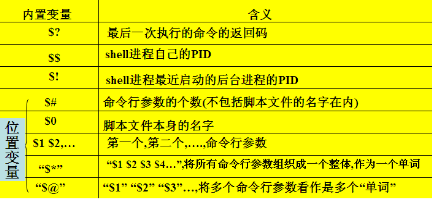
\includegraphics[width=9cm,height=4.5cm]{c8.shell.buildin.01.png}}
	  \item 赋值:使用=(赋值运算符),=两边不能有空格,在=后面跟一个换行符赋空值
	  \item 访问:默认情况下将变量视作文本字符串,在变量名前加\$可以访问变量的值 
	  \item 变量名:只能包含字母、数字和下划线,必须以字母或下划线开头,大小写敏感(惯例使用大写)
	\end{itemize}
      \item 从键盘读取输入:使用read读取键盘输入并为变量赋值
      \item 特殊变量
      \item 退出状态:0表示成功,1表示不成功
    \end{enumerate}

  \item
    \textcolor{red}{\textbf{【重点、难点】}}流程控制(20分钟)\textcolor{red}{(结合逻辑流程讲解语法结构,并进行实例分析)}
    \begin{enumerate}
      \item 简介
	\begin{itemize}
	  \item 流程控制允许程序做出判断:程序计算条件的值,并根据这些条件执行相应的操作
          \item 条件流程控制:根据特定的约束是否满足来决定是否执行某个代码段
          \item 迭代流程控制:代码块重复或迭代,直到满足某个条件为止
	\end{itemize}

    \vspace*{-10pt}
    \begin{figure}[h]
      \centering
      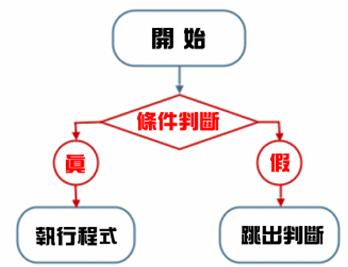
\includegraphics[width=5.5cm]{c8.conditional.01.jpg}
      \quad
      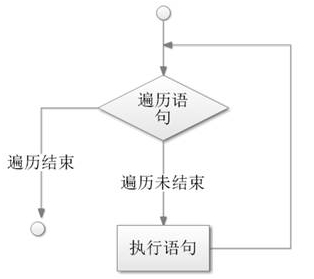
\includegraphics[width=5.5cm]{c8.iterative.jpg}
    \end{figure}
    \vspace*{-10pt}


\otherTail
\newpage
\otherHeader


      \item 条件流程控制
	\begin{itemize}
	  \item if-then
	    \begin{itemize}
	      \item if-then
\parpic[fr]{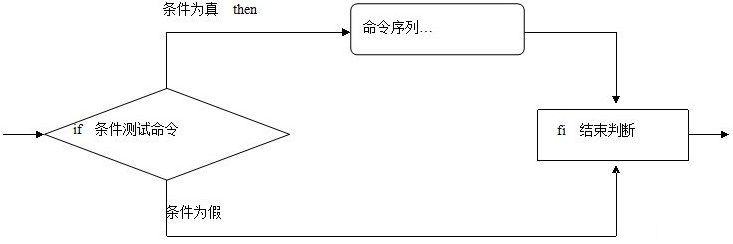
\includegraphics[width=8cm,height=2cm]{c8.if.01.jpg}}
\begin{verbatim}
if some_condition
then
  something happens
fi
\end{verbatim}
	      \item if-then-else
\parpic[fr]{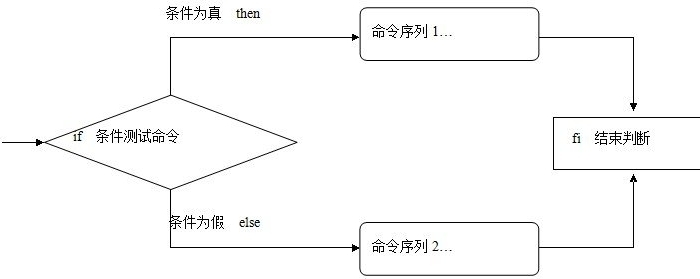
\includegraphics[width=8cm]{c8.if.02.jpg}}
\begin{verbatim}
if some_condition
then
  something happens
else
  something happens
fi
\end{verbatim}
	      \item if-then-elif-else
\parpic[fr]{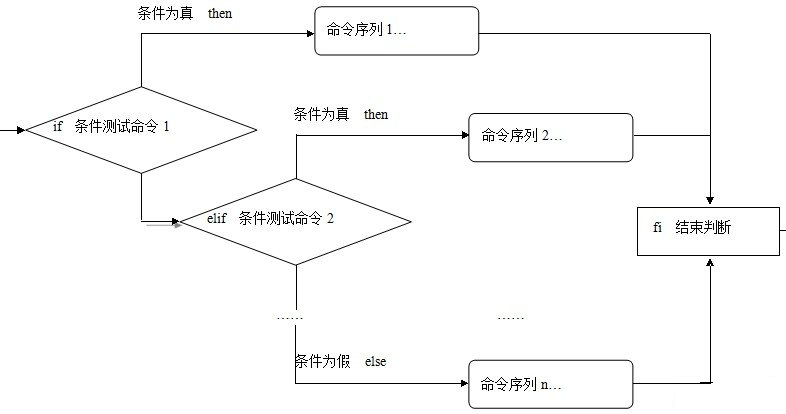
\includegraphics[width=8cm]{c8.if.03.jpg}}
\begin{verbatim}
if some_condition
then
  something happens
elif other_condition
  something happens
else
  something happens
fi
\end{verbatim}
	    \end{itemize}

	  \item test
\parpic[fr]{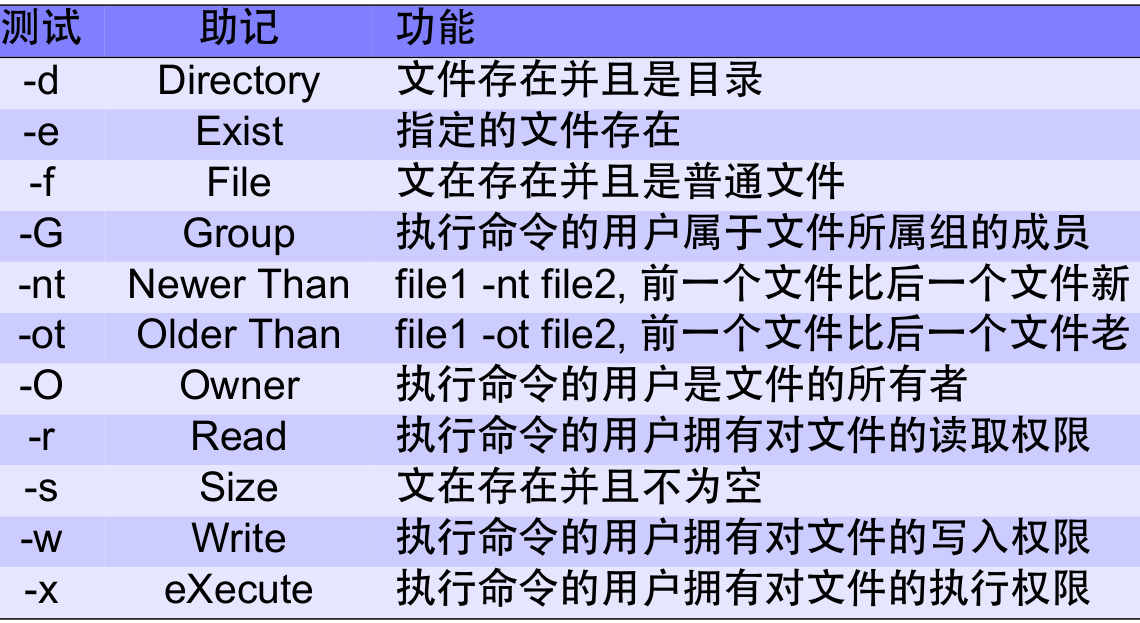
\includegraphics[width=8cm]{c8.test.png}}
	    \begin{itemize}
	      \item 语法
\begin{verbatim}
# 注意中括号内的空格
if [ $COLOR="purple" ]
if (test $COLOR="purple")
# 测试文件是否存在
if [ -e filename ]
if (test -e filename)
\end{verbatim}
	      \item 文件测试
	    \end{itemize}

	  \item 比较运算符
	    \begin{itemize}
\parpic[fr]{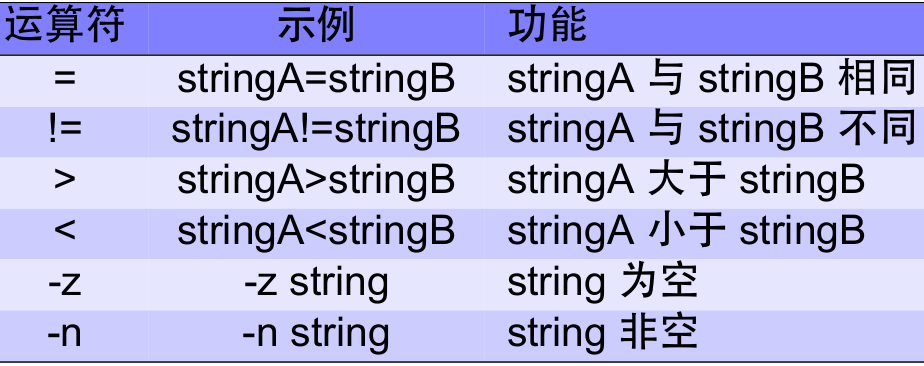
\includegraphics[width=8cm]{c8.compare.01.png}}
	      \item 字符串比较
	      \item 整数值比较
	    \end{itemize}

          \item 多个条件
	      \begin{itemize}
		\item 逻辑运算符and(\&\&)
\begin{verbatim}
if [ cond1 && cond2 ]
then
  some action
fi
\end{verbatim}
\vspace*{-10pt}
\begin{figure}[h]
\parpic[fr]{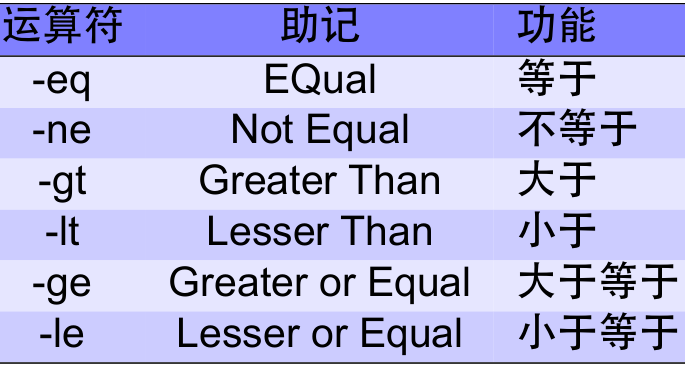
\includegraphics[width=6cm]{c8.compare.02.png}}
\end{figure}
\vspace*{-10pt}
\begin{verbatim}
# 等价于
if [ condition1 ]
then
  if [ condition2 ]
  then
    some action
  fi
fi
\end{verbatim}


\otherTail
\newpage
\otherHeader


		\item 逻辑运算符or(||)
\parpic[fr]{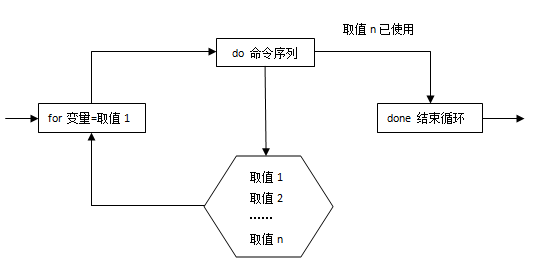
\includegraphics[width=9cm]{c8.for.01.png}}
\begin{verbatim}
if [ cond1 || cond2 ]
then
  some action
fi
# 等价于
if [ condition1 ]
then
  some action
elif [ condition2 ]
then
  the same action
fi
\end{verbatim}
	      \end{itemize}

	  \item case
\parpic[fr]{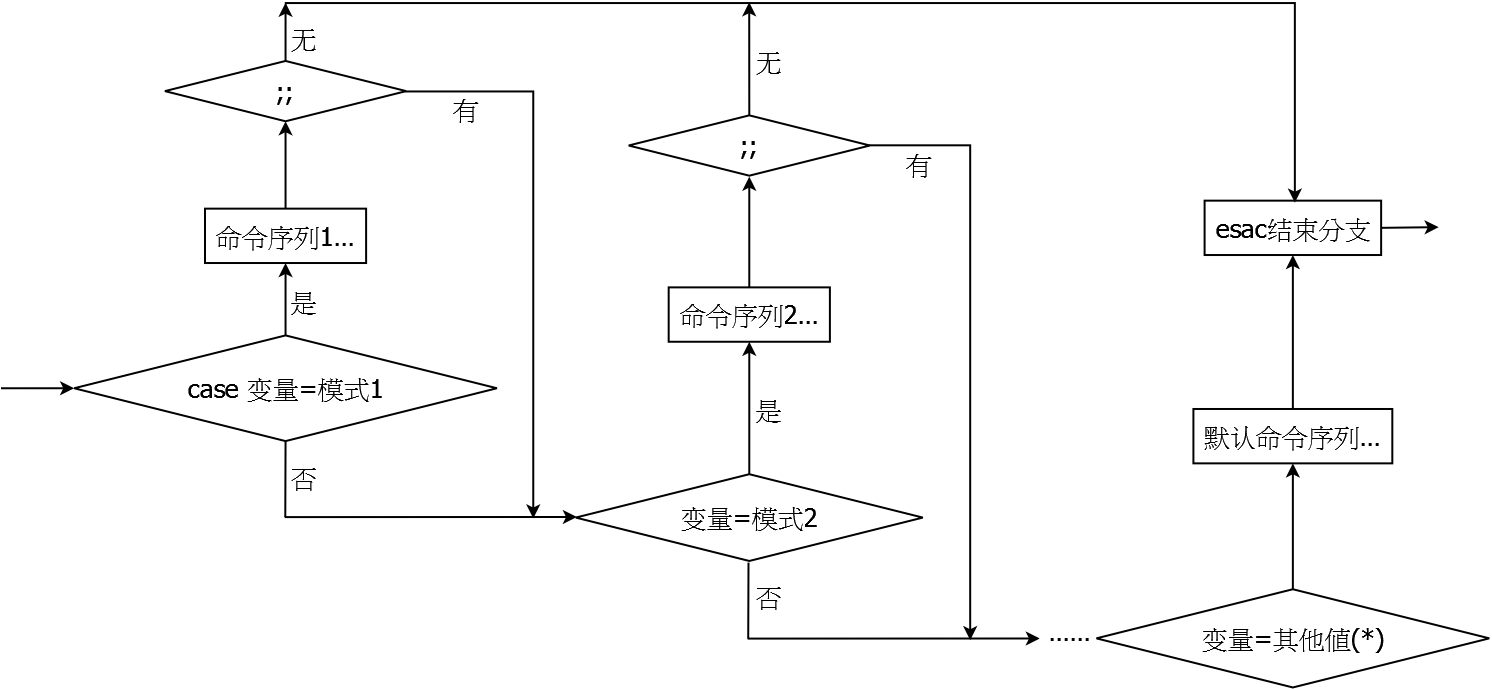
\includegraphics[width=11cm]{c8.case.01.png}}
\begin{verbatim}
case expression in
  pattern1)
    action1
    ;;
  pattern2)
    action2
    ;;
  *)
    default action
    ;;
esac
\end{verbatim}

	\end{itemize}

      \item 迭代流程控制
\parpic[fr]{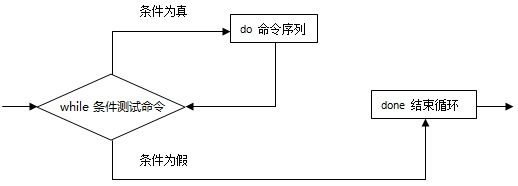
\includegraphics[width=8.5cm]{c8.while.01.png}}
	\begin{itemize}
	  \item while
\begin{verbatim}
while condition
do
  action
done
\end{verbatim}

	  \item until
\parpic[fr]{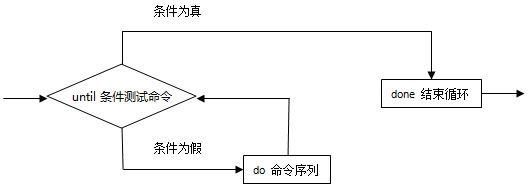
\includegraphics[width=8.5cm]{c8.until.01.png}}
\begin{verbatim}
until condition
do
  action
done
\end{verbatim}
	  \item for
\begin{verbatim}
for VAR in LIST
\end{verbatim}
\parpic[fr]{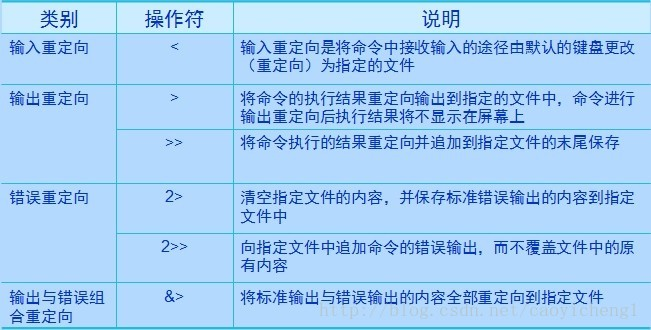
\includegraphics[width=10cm]{c8.std.01.jpg}}
\begin{verbatim}
do
  action
done
\end{verbatim}
	\end{itemize}
    \end{enumerate}

  \item 高级概念(10分钟)
    \begin{enumerate}
      \item 输入输出重定向
      \item 命令替换
	\begin{itemize}
	  \item \verb|``|
	  \item \verb|$()|
	\end{itemize}
    \end{enumerate}


\otherTail
\newpage
\otherHeader


  \item
    \textcolor{red}{\textbf{【难点】}}shell函数(30分钟)\textcolor{red}{(实例分析、操作演示)}
    \begin{enumerate}
      \item 声明与调用
	\vspace*{-10pt}
	\begin{multicols}{2}
\begin{verbatim}
# 函数声明
name () {
  commands
}
# 函数调用,不带()
name
name parameter(s)
\end{verbatim}
\begin{verbatim}
#!/bin/bash
# A simple function
repeat () {
  echo "I don't know $1 $2"
}
repeat Your Name
# I don't know Your Name
\end{verbatim}
	\end{multicols}
	\vspace*{-10pt}
      \item 返回值:默认是最后一条语句的状态,可以使用return显式地设置函数的退出状态
      \item 嵌套和递归
	\begin{itemize}
	  \item 递归函数:就像调用其他函数一样、调用自己的函数
	  \item 函数嵌套:在一个函数中调用包含在另一个函数中的功能
	\end{itemize}
      \item 文件处理
	\vspace*{-5pt}
\begin{verbatim}
if [ -r File && -x File  ]
then
  echo "File exists, is readable, and executable!"
fi
if [ -r File || -w File  ]
then
  echo "File exists and is readable or writable!"
fi
\end{verbatim}
	\vspace*{-5pt}
      \item 作用域
	\begin{itemize}
	  \item 全局作用域:在脚本的任何地方都可以访问变量
	  \item 局部作用域:只能在声明变量的作用域内访问它们
	  \item 使用local关键字定义局部变量
	\end{itemize}
      \item 数组
	\begin{itemize}
	  \item 声明
	\vspace*{-5pt}
	    \begin{itemize}
	      \item \verb|array[index]=value|
	      \item \verb|array2=(value1 value2 value3 ...)|
	      \item \verb|array3=([0]=value1 [13]=value2 [7]=value3)|
	    \end{itemize}
	  \item 解引用数组
	    \begin{itemize}
	      \item 获得数组中某个特定索引位置的数据:\verb|${array[index]}|
	      \item 获得数组中的所有数据:\verb|arrayElements=${array[@]}|
	      \item 获得数组包含的元素数目:\verb|arrayLength=${#array[@]}|
	      \item 获得数组中包含的索引值:\verb|arrayIndex=${!array[@]}|
	      \item 获得第四个元素(含)之后的所有元素的数据:\verb|afterTue=${day[@]:3}|
	      \item 获得第四个元素(含)后面两个元素的数据:\verb|WedThu=${day[@]:3:2}|
	    \end{itemize}
	  \item 删除数组
	    \begin{itemize}
	      \item 删除索引位置为1的元素的数据:\verb|unset array[1]|
	      \item 删除数组中所有元素的数据:\verb|unset array[@]|
	    \end{itemize}
	\end{itemize}
    \end{enumerate}

  \item 脚本调试(5分钟)
    \begin{itemize}
      \item \verb|sh -n script|:检查语法,不执行脚本。
      \item \verb|sh -x script|:执行脚本并显示所有变量的值。
      \item \verb|set -x; command; set +x|:脚本局部调试。
      \item \verb|echo|:打印变量的值、提示信息等来调剂脚本。
    \end{itemize}


\otherTail
\newpage
\otherHeader


  \item 总结与答疑(5分钟)
    \begin{enumerate}
      \item 知识点
	\begin{itemize}
          \item shell脚本编程起步:脚本结构、运行、注释,调用shell,变量、特殊变量,从键盘读取输入,退出状态
          \item 条件流程控制:if-then,test,case
          \item 迭代流程控制:while,until,for
          \item shell编程高级概念:输入输出重定向,命令替换
          \item shell函数:声明与调用,返回值,嵌套和递归,作用域,文件处理,数组
          \item shell脚本的调试
	\end{itemize}
      \item 技能
	\begin{itemize}
          \item 掌握shell编程的基本语法和调试命令
          \item 使用shell编写应用脚本
	\end{itemize}
    \end{enumerate}

\end{enumerate}

\otherTail



\end{document}

